\chapter{固定翼无人机飞控建模}\label{routing}
本文进行固定翼无人机飞控建模,选择c172p飞机。固定翼飞机与四旋翼飞机在空气动力学特性等方面存在着很多不同。本文采用FlightGear自带的JSBSim飞行动力学模型,进行固定翼飞机的飞行控制,如图\ref{fig40}所示。
\vspace{-10pt}
\begin{figure}[!ht]
\centering
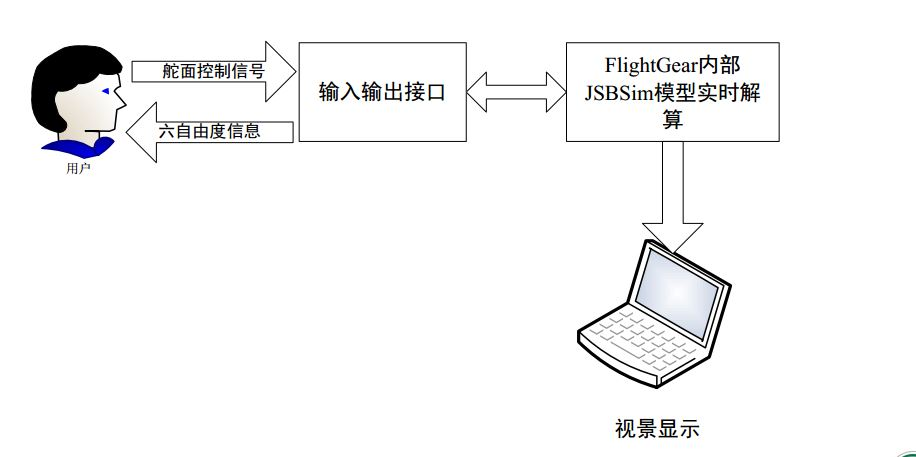
\includegraphics[width=0.8\textwidth]{f33.jpg}
\caption{固定翼飞控建模过程}
\label{fig40}
\end{figure}
\vspace{-10pt}
\section{JSBSim介绍}
JSBsim 是一个通用的 6 自由度动态模型,模拟飞行工具的运动。它使用 C++语言编写,可以运行在单机方式下,也可以驱动有视觉子系统的大型程序。YAsim是由 Andrew Ross 开发的新动力学模型,是 Flightgear 的集成部分,它通过模拟飞行器不同部分的气流来实现,这点不同于 JSBsim。UIUC 飞行动态模型是基于LaRCsim 的,最初是 NASA 开发的,通过使用飞行器配置文件来扩充代码\ucite{28}。目前 JSBsim\ucite{29}和 UIUC 是比较流行的动力学仿真系统,并且均是开源项目。

\section{JSBSim飞行动力学模型}
根据FlightGear自带的JSBSim飞行控制模型,进行飞行控制。包括飞机舵面的控制,飞机姿态的控制。
\begin{itemize}
  \item 升降舵控制

  升降舵主要控制飞机的俯仰姿态运动,在JSBSim中对升降舵控制的代码如下:
   \begin{lstlisting}[language==XML]
<flight_control name="FCS:c172p">
<channel name="All">
    <summer name="Pitch Trim Sum">
        <input>fcs/elevator-cmd-norm</input>
        <input>fcs/pitch-trim-cmd-norm</input>
        <clipto>
            <min>-1</min>
            <max>1</max>
        </clipto>
</summer>
<aerosurface_scale name="Elevator Control">
    <input>fcs/pitch-trim-sum</input>
        <range>
            <min>-0.35</min>
            <max>0.3</max>
        </range>
    <output>fcs/elevator-pos-rad</output>
</aerosurface_scale>
 \end{lstlisting}
  \item 方向舵控制

  方向舵主要控制飞机的偏航运动,在小飞机转弯的过程中,起着重要的作用。JSBSim的代码如下:
  \begin{lstlisting}[language==XML]
<summer name="Rudder Command Sum">
    <input>fcs/rudder-cmd-norm</input> 
    <input>fcs/yaw-trim-cmd-norm</input>
    <clipto>
        min>-1</min>
        <max>1</max>
    </clipto>
</summer>
<aerosurface_scale name="Rudder Control">
    <input>fcs/rudder-command-sum</input>
        <range>
            <min>-0.35</min>
            <max>0.35</max>
        </range>
    <output>fcs/rudder-pos-rad</output>
</aerosurface_scale>
 \end{lstlisting}
  \item 副翼控制
  
  副翼主要控制飞机的滚转运动,副翼分为左右副翼,JSBSim控制代码如下:
    \begin{lstlisting}[language==XML]
<summer name="Roll Trim Sum">
    <input>fcs/aileron-cmd-norm</input>
    <input>fcs/roll-trim-cmd-norm</input>
        <clipto>
            <min>-1</min>
            <max>1</max>
        </clipto>
</summer>
<aerosurface_scale name="Left Aileron Control">
    <input>fcs/roll-trim-sum</input>
        <range>
            <min>-0.35</min>
            <max>0.35</max>
        </range>
    <output>fcs/left-aileron-pos-rad</output>
</aerosurface_scale>
<aerosurface_scale name="Right Aileron Control">
    <input>-fcs/roll-trim-sum</input>
        <range>
            <min>-0.35</min>
            <max>0.35</max>
        </range>
    <output>fcs/right-aileron-pos-rad</output>
</aerosurface_scale>
 \end{lstlisting}
\end{itemize}

本文选择c172p飞机,如图\ref{fig41}所示,结合上面JSBsim模型对c172p进行飞行控制。

\begin{figure}[!ht]
\centering
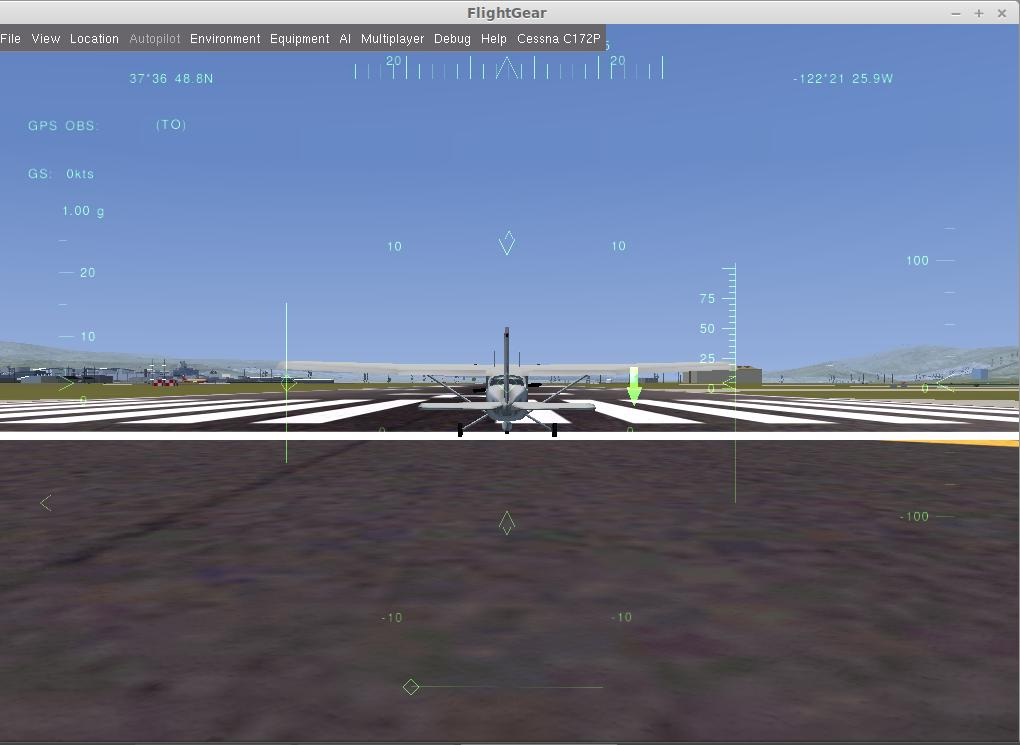
\includegraphics[width=0.6\textwidth]{f34.jpg}
\caption{固定翼飞控建模过程}
\label{fig41}
\end{figure}


